\subsection{Функция стохастический чувствительности}
    
    Функция стохастический чувствительности это инструмент, который показывает... 

    \comment{Думаю формулы тут не нужны, мб оставить ссылку на статью Crises, noise, and tipping in the Hassell population model}

    Давайте посмотрим на график \ref{bifurcation_x_0_2_a_1_beta_chaos_fss}. Красными линиями нарисована функция стохастический чувствительности. \comment{напиши зачем она тут вообще нужна}. 

    % \begin{figure}
    %     \centering
    %     \includegraphics[width=\textwidth]{stochastic/bifurcation_x_0_2_a_1_beta_noise_fss.jpg}
        
    %     \captionsetup{justification=centering}
    %     \caption{График бифуркации с \(\beta\)-шумом.}
    %     \label{bifurcation_x_0_2_a_1_beta_chaos_fss}
    % \end{figure}

    \begin{figure}
        \centering
        \subfloat[Для модели (\ref{origin})]{
            \includegraphics[width=0.7\textwidth]{stochastic/images/bifurcation_x_0_2_a_1_beta_noise_fss.jpg}
            \label{bifurcation_x_0_2_a_1_beta_chaos_fss}
        }

        \subfloat[Для модели (\ref{alpha_chaos})]{
            \includegraphics[width=0.5\textwidth]{stochastic/images/bifurcation_x_0_2_a_1_beta_noise_fss_segment_stable.jpg}
            \label{bifurcation_x_0_2_a_1_beta_chaos_fss_segment_stable}
        }  
        \subfloat[Для модели (\ref{beta_chaos})]{
            \includegraphics[width=0.5\textwidth]{stochastic/images/bifurcation_x_0_2_a_1_beta_noise_fss_segment_2_cycle.jpg}
            \label{bifurcation_x_0_2_a_1_beta_chaos_fss_segment_2_cycle}
        }
            
        \subfloat[Для модели (\ref{additive_chaos})]{
            \includegraphics[width=0.5\textwidth]{stochastic/images/bifurcation_x_0_2_a_1_beta_noise_fss_segment_chaos_up.jpg}
            \label{bifurcation_x_0_2_a_1_beta_chaos_fss_segment_chaos_up}
        }
        \subfloat[Для модели (\ref{additive_chaos})]{
            \includegraphics[width=0.5\textwidth]{stochastic/images/bifurcation_x_0_2_a_1_beta_noise_fss_segment_chaos_down.jpg}
            \label{bifurcation_x_0_2_a_1_beta_chaos_fss_segment_chaos_down}
        }
            
        \caption{Временные ряды при \(\alpha = 1, \beta = 0.56, x_0 = 0.06, \varepsilon = 0.004\)}
    \end{figure}

    Рассмотрим участок от \(\beta \approx 0.45\) до \(\beta \approx 0.48\), он изображен на рисунке \ref{bifurcation_x_0_2_a_1_beta_chaos_fss_segment_stable}. Мы видим, что значения графика бифуркации почти всегда находятся в коридоре, границами которого являются значения ФСЧ. Этот коридор строится по правилу трех сигм. Такой подход гарантирует, что почти все значения будут находиться в этом интервале, что собственно мы и наблюдаем.

    % \begin{figure}
    %     \centering
    %     \includegraphics[width=\textwidth]{stochastic/bifurcation_x_0_2_a_1_beta_noise_fss_segment_stable.jpg}
        
    %     \captionsetup{justification=centering}
    %     \caption{}
    %     \label{bifurcation_x_0_2_a_1_beta_chaos_fss_segment_stable}
    % \end{figure}

    На участках с k-циклами и хаосом (рисунки \ref{bifurcation_x_0_2_a_1_beta_chaos_fss_segment_2_cycle}, \ref{bifurcation_x_0_2_a_1_beta_chaos_fss_segment_chaos_up} и \ref{bifurcation_x_0_2_a_1_beta_chaos_fss_segment_chaos_down]}) будет наблюдаться аналогичная ситуация: значения лежат в коридоре, ограниченном значениями ФСЧ.

    % \begin{figure}
    %     \centering
    %     \includegraphics[width=\textwidth]{stochastic/bifurcation_x_0_2_a_1_beta_noise_fss_segment_2_cycle.jpg}
        
    %     \captionsetup{justification=centering}
    %     \caption{}
    %     \label{bifurcation_x_0_2_a_1_beta_chaos_fss_segment_2_cycle}
    % \end{figure}

    % \begin{figure}
    %     \centering
    %     \includegraphics[width=\textwidth]{stochastic/bifurcation_x_0_2_a_1_beta_noise_fss_segment_chaos_up.jpg}
        
    %     \captionsetup{justification=centering}
    %     \caption{}
    %     \label{bifurcation_x_0_2_a_1_beta_chaos_fss_segment_chaos_up}
    % \end{figure}

    % \begin{figure}
    %     \centering
    %     \includegraphics[width=\textwidth]{stochastic/bifurcation_x_0_2_a_1_beta_noise_fss_segment_chaos_down.jpg}
        
    %     \captionsetup{justification=centering}
    %     \caption{}
    %     \label{bifurcation_x_0_2_a_1_beta_chaos_fss_segment_chaos_down}
    % \end{figure}

    \comment{напиши что-нибудь про ФСЧ}